\documentclass{article}
\usepackage{geometry}[a4paper, margin=2in]
\usepackage{graphicx}
\title{Practical Submission Sheet}
\newcommand{\bb}[1]{\textbf{#1}}
\date{}
\begin{document}
	\maketitle
	\begin{tabular}{ll}
		\bb{Term}: 2020-1 & \bb{Submission Date}: \today\\
		\bb{Lecture Date}: August 14, 2020. & \bb{Practical Number}: 2\\
		\bb{Course Code}: PHY249 & \bb{Section}: G2903\\
		\bb{Registration Number}: 11912610 & \bb{Roll No}: 03\\
		\bb{Student Name}: Aayush Arya & \\
	\end{tabular}
	
	\section*{Concepts Learnt}
	Learnt what different types of transitors exist (npn and pnp transitors) and how to connect them in different configurations (common emitter, base and collector). Gained the operational ability to complete a common emitter transistor circuit. 
	\section*{Key Observations \& Insights}
	For the simulated diode we tested, the plot for V-I characteristics obtained was as expected \textemdash the knee and ohmic regions were clearly identifiable. In the case of the transistor, the behavior of current flow was observed.
	\section*{Application Areas}
	Diodes are useful for restricting current in one direction. This may be desirable in many electrical circuits. Transitors are used as switches and current amplifiers. They are very common in electronic devices, especially computers.
	\section*{Report}
	A diode circuit was made using a $1k\Omega$ resistor and an LED for the purpose of testing, as depicted in circuit\_diode.png (see folder). Both the LED and resistor provided resistance in the circuit and consequently were useful in restricting the maximum current that passes through the diode.
	
	The current and voltage profiles of the simulated diode were recorded. The observations are summarised in Table 1.
	\begin{table}[!h]
		\begin{center}
			\begin{tabular}{|c|c|c|c|}
				\hline
				Voltage (V) & 	& I (mA) & \\
				\hline
				1.0 & 5.5 & 0.001 & 2.835 \\
				1.5 & 6.0 & 0.026 & 3.792 \\
				2.0 & 6.5 & 0.216 & 4.274 \\
				2.5 & 7.0 & 0.572 & 4.758 \\
				3.0 & 7.5 & 0.990 & 5.244 \\
				3.5 & 8.0 & 1.436 & 5.731 \\
				4.0 & 8.5 & 1.895 & 6.219 \\
				4.5 & 9.0 & 2.362 & 6.707\\
				5.0 &	& 3.312 & \\
				\hline
			\end{tabular}
			\caption{Applied voltage and corresponding current across the diode}
		\end{center}
	\end{table}


	The corresponding plot with current (mA) on the vertical axis and applied voltage (V) on the horizontal axis is as displayed in Figure 1. The plot was generated using matplotlib (Python).\\
	\begin{figure}[!h]
		\begin{center}
			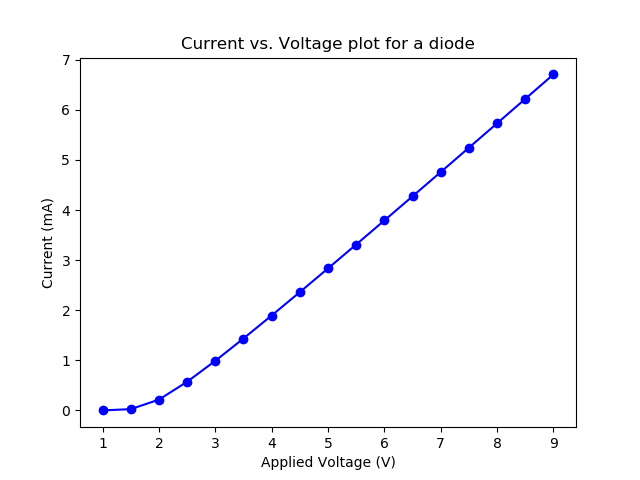
\includegraphics[width=0.75\textwidth]{plot_diode.png}
		\end{center}
		\caption{The V-I characteristic of the diode.}
	\end{figure}
	
	
	An npn transistor was simulated and was connected in common emitter configuration with two $100\Omega$ resistors and two battery sources of $5V$ each. The circuit for the transistor is as reported in \textit{circuit\_transistor.png}.\\
	The resulting behavior was as expected for an npn transistor, with a net current flowing into the collector and flowing out of the emitter.
\end{document}